\chapter{Results and Discussion}
The starting point of this project was the interdigitated qubit (see figure \ref{fig:Yale_parameters2}). This chapter will start with a discussion of the results gathered on this design.
%\cite{Houck2007}
%%The main focus during this project rested on two distinct qubit designs, namely the interdigitated and the parallel pad qubits. The two designs can be compared in figure \ref{fig:}.


First, the influence of different parameters on the capacitance of structures was determined. This knowledge enables designing structures with a specific capacitance necessary for a qubit with a certain frequency (see equation \eqref{eq:ResonanceFrequency}). The target capacitance is 60 \(f\)F. With an inductor having an inductance of 10 \(n\)H this result in a resonance frequency of around 6.5 \(G\)Hz. \todo{HOW is the capacitance retrieved? refer to appendix?}


Secondly, the participation ratio of the lossy layers is determined. This will give insight into what design decisions can be made to reduce these participation ratios.\\
Taking these insights into account, a second qubit design was investigated in similar fashion. 

\vfill

\begin{figure}[h]
	\centering
	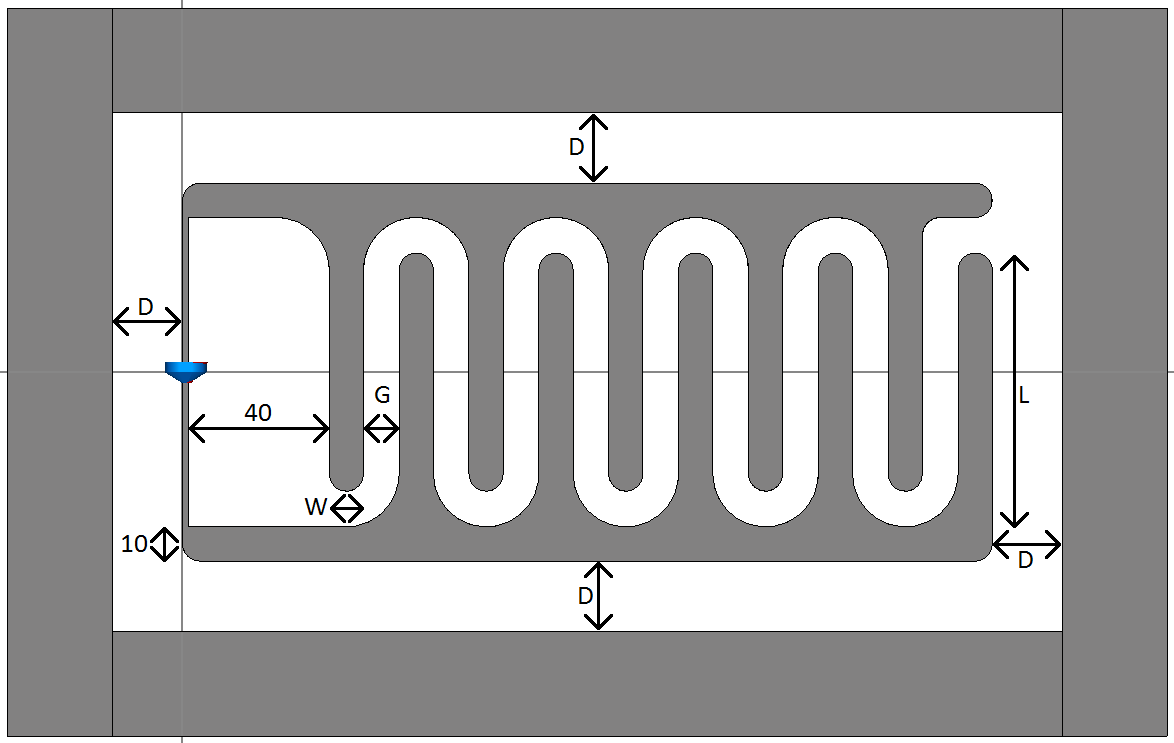
\includegraphics[scale = .4]{Figures/Yale_parameters2_cropped}
	\caption{The interdigitated qubit design including parameters and dimensions valid for all iterations of the design. (D) is the separation of the ground plane, (L) is the length of the fingers, (G) is the gap between the fingers, and (W) is the width of the fingers. Dimensions are in micrometers.}
	\label{fig:Yale_parameters2}
\end{figure}

\clearpage
\section{Interdigitated qubit}
As the name suggests the interdigitated qubit consists of two pads having a certain amount of fingers. The pads are positioned such that the gap between the two pads is of equal size (G) along all fingers. The distance between the Josephson junction and the first finger was set to 40 \(\mu\)m for all interdigitated qubit designs. The width (W) of the fingers is always kept equal to the gap (G) between the fingers. The distance between the pads and the groud (D) is the same on all sides. The last parameter is the length (L) of the fingers. An overview of the design with its parameters is depicted in figure \ref{fig:Yale_parameters2}.

\subsection{The capacitance}
The capacitance of the system is retrieved by a separate simulation, detailed in appendix \ref{appendix:CST_procedure}. It is used to calculate the total energy stored the qubit at resonance (see equation \eqref{eq:totalenergy}).
To better determine the influence of the pad design on the capacitance of the system, the influence of the ground plane is determined as a function of separation distance. Figure \ref{fig:capacitance_vs_slotsize} shows the capacitance of the qubit as a function of the separation distance of the ground plane (D). It indicates that the influence of the ground plane on the capacitance of the system decreases rapidly with increasing separation distance. The influence of the ground plane becomes insignificant only at a separation distance of around 100 \(\mu\)m. So, in order to determine the influence of changes in pad design on the capacitance (and participation ratio) of the system, the separation distance of the ground plane should be carefully kept equal among pad designs. \todo{Or I should have eliminated the ground plane altogether when determining the influence of certain parameters.} 

\begin{figure}
	\centering
	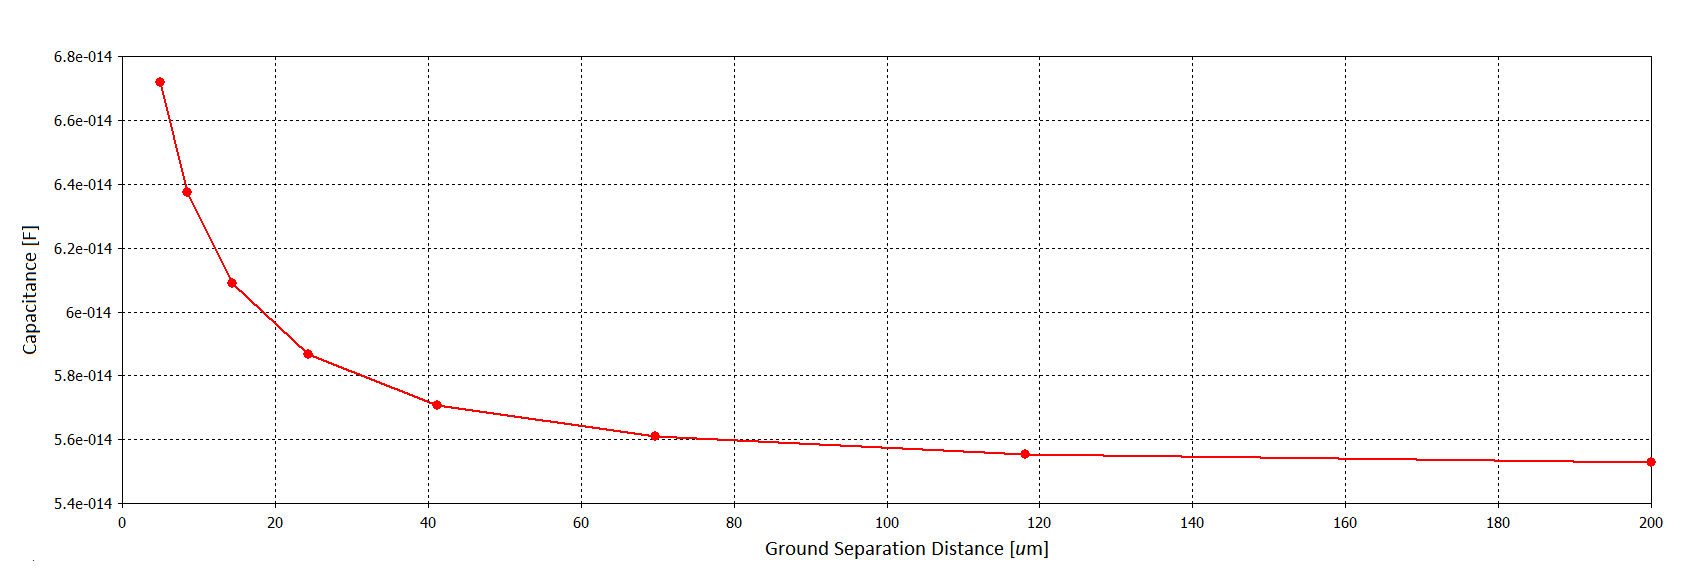
\includegraphics[width = \textwidth]{Figures/capacitance_vs_slotsize_edit}
	\caption{Capacitance of the system as a function of ground plane separation (D in figure \ref{fig:Yale_parameters2})}
	\label{fig:capacitance_vs_slotsize}
\end{figure}

For the interdigitated pad design specifically, the first parameter under investigation is the amount of 'fingers' in the  qubit. The capacitances of qubits with 4 to 9 fingers were determined. The finger length (\(L=56\mu m\)), width and gap (\(W=G=20\mu m\)) were not changed.
As can be seen in figure \ref{fig:CapVSFingers} where the capacitance of systems with 4 to 9 fingers has been depicted, the relationship appears to be linear. This can be explained by viewing the addition of a finger as the addition of an extra capacitor in parallel.

\begin{figure}
	\centering
	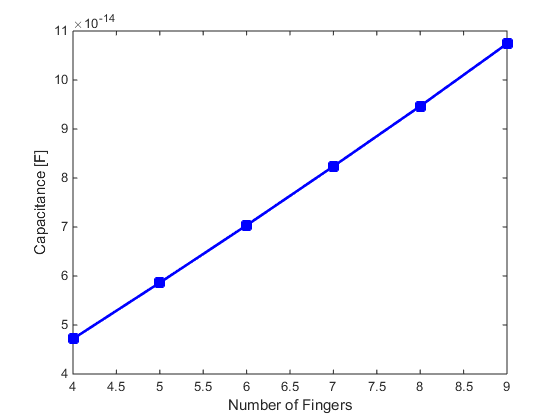
\includegraphics[scale = 0.7]{Figures/Capacitance_Plots/CapVSFingers.png}
	\caption{Capacitance as a function of the amount of fingers in the interdigitated qubit design. The finger length (\(L=56\mu m\)), width and gap (\(W=G=20\mu m\)) were not changed.}
	\label{fig:CapVSFingers}
\end{figure}

Next the influence of the finger width (W) is determined. The finger separation (G) is kept equal to the finger width. For a design with five fingers (\(L=56\mu m\)) and ground separation distance \(D = 20\mu m\), the finger width was changed between \(5\) and \(50\mu m\). The resulting capacitances are depicted in figure \ref{fig:CapVSWidthL10}. This relationship also appears to be linear.

\begin{figure}
	\centering
	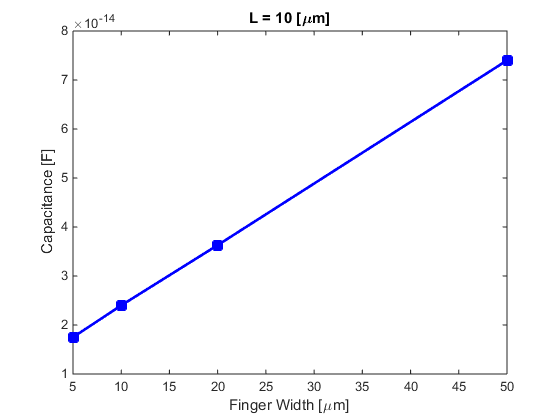
\includegraphics[scale = 0.7]{Figures/Capacitance_Plots/CapVSWidthL10.png}
	\caption{Capacitance as a function of finger width in the interdigitated qubit design. The finger separation (G) is kept equal to the finger width. All qubit have five fingers and equal finger length (\(L=56\mu m\)).}
	\label{fig:CapVSWidthL10}
\end{figure}

Having determined the dependencies, qubits can be designed to have specific capacitances. Keeping all other parameters equal, the capacitance of earlier systems was tuned by adjusting the length of the fingers. For qubits with 5 fingers and a finger width of 5 to 50 \(\mu\)m, and a ground separation distance \(D = 20\mu m\), the finger length was adjusted between 10 and 100 \(\mu\)m. \\
The results are combined in figure \ref{fig:Capacitances_g5_50}. It shows the capacitance as a function of finger length (L) for systems with a finger width (W) of 5, 10, 20, and 50 \(\mu\ m\). From the figure it is possible to determine the finger length needed to achieve the target capacitance of 60 \(f\)F. For qubits with a finger width of  5 \(\mu\)m, 10 \(\mu\)m, and 20 \(\mu\)m, their length must be 87 \(\mu\)m, 76 \(\mu\)m, and 56 \(\mu\)m  respectively.   

\begin{figure}
	\centering
	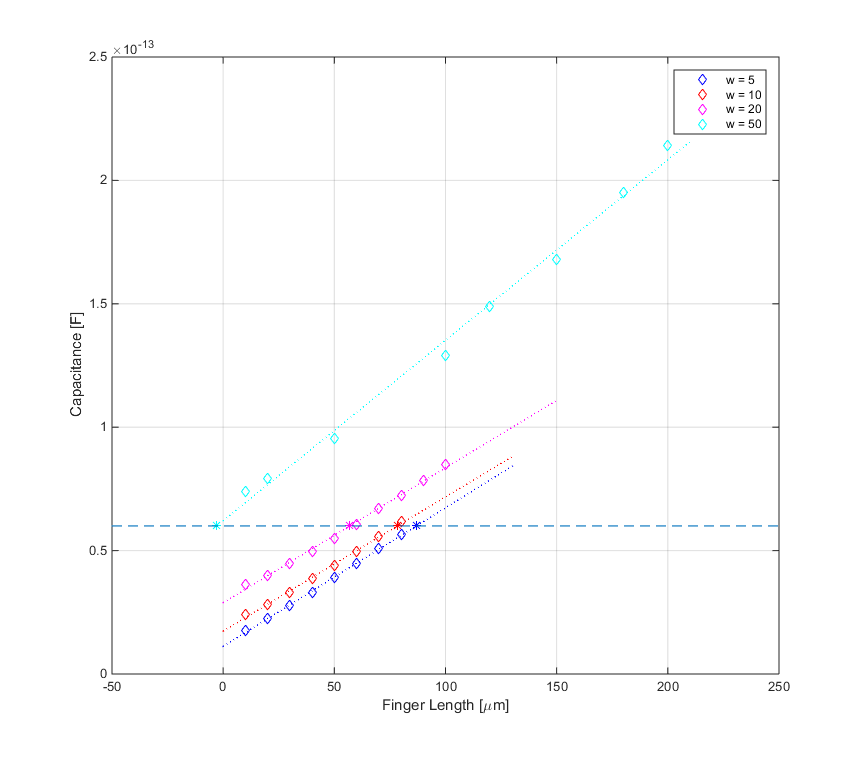
\includegraphics[width = \textwidth]{Figures/Capacitances_g5_50}
	\caption{The capacitance as a function of finger length for several finger widths. The ground separation distance (D) is \(20\mu m\). The finger length was adjusted between 10 and 100 \(\mu\)m. Dotted lines represent linear fits of the data. The horizontal dashed line is a guideline for the eye showing the necessary finger length to make a 60\(f\)F capacitor; 87 \(\mu\)m, 76 \(\mu\)m, and 56 \(\mu\)m for qubits with a finger width of  5 \(\mu\)m, 10 \(\mu\)m, and 20 \(\mu\)m respectively.}
	\label{fig:Capacitances_g5_50}
\end{figure} 

\clearpage

 \begin{figure}
 	\centering
 	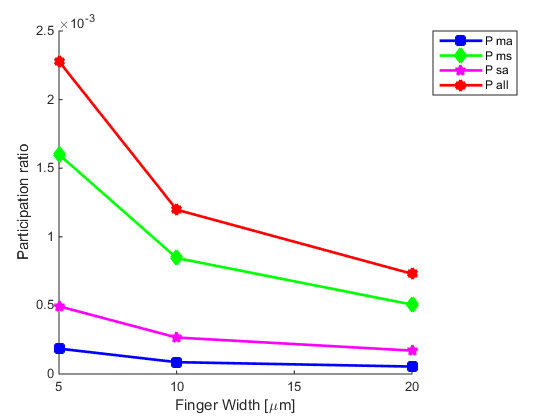
\includegraphics[scale = 0.7]{Figures/Ratio_plots/FingerWidth_legend}
 	\caption{A plot of the different ratios for qubits with five fingers. The length of the fingers has been adjusted for each qubit to reach a capacitance of 60 \(f\)F. For qubits with a finger width of  5 \(\mu\)m, 10 \(\mu\)m, and 20 \(\mu\)m, their lengths are 87 \(\mu\)m, 76 \(\mu\)m, and 56 \(\mu\)m  respectively. The ground separation distance (D) is \(20\mu m\).}
 	\label{fig:FingerWidth_legend}
 \end{figure}

\subsection{The participation ratios}
Using the previous results several interdigitated qubits were designed to have a capacitance of 60 \(f\)F. Together with an inductance of 10 \(n\)H the target resonance frequency is 6.5 \(G\)Hz (see equation \eqref{eq:ResonanceFrequency}). An overview of the relevant parameters can be seen in table \ref{table:60fF_fingerlength}. For all qubit designs the ground separation distance (D) is \(20 \mu m\). The resulting participation ratios of the different lossy layers can be seen in the same table. For the qubit with 5 fingers they are also plotted as a function of finger width (W) in figure \ref{fig:FingerWidth_legend}. As the finger width is increased and the finger length decreased, all participation ratios decrease.

\begin{table}
	\begin{center}
		\begin{tabular}{ | l || c | c || c | c | c | c |}
			\hline
			Fingers  & Finger Width [\(\mu\)m] & Finger Length [\(\mu\)m]  & P ma &  Pms & P sa & P all \\ \hline
			5 & 5 & 87 & 1.85e-04 & 1.60e-03 & 4.94e-04 & 2.28e-03 \\  
			5 & 10 & 76 & 8.62e-05 & 8.45e-04 & 2.66e-04 & 1.20e-03 \\
			5 & 20 & 56 & 5.43e-05 & 5.06e-04 & 1.70e-04 & 7.31e-04  \\
			10 & 5 & 36 & 1.36e-04 & 1.30e-03 & 4.12e-04 & 1.85e-03 \\
			10 & 10 & 26 & 7.56e-05 & 7.33e-04 & 2.46e-04 & 1.06e-03 \\
			\hline
		\end{tabular}
	\end{center}
	\caption{The relevant parameters for interdigitated qubit and the resulting participation ratios. For all designs the finger length has been tuned to result in a qubit with a capacitance of 60 \(f\)F. }
	\label{table:60fF_fingerlength}
\end{table}



By default the corners of the fingers were rounded (as in figure \ref{fig:Yale_parameters2}). As this was not standard practice the influence of doing so was determined retroactively. To do so the corner radius of the fingers (with a width of 20 \(\mu\)m) was changed between 1 and 10 \(\mu\)m (10 \(\mu\)m making semi-circles at the finger tips). The qubit had 5 fingers with a width (W) and gap (G) of \(20 \mu m\), a finger length (L) of \(56 \mu m\), and a pad separation distance (D) of \(20 \mu m\). The resulting participation ratios can be seen in table \ref{table:ratio_cornerradius} and figure \ref{fig:CornerRadius} as a function of corner radius. All participation ratios tend to decrease as the corner radius is increased. The retrieved participation ratios for a corner radius of 8 \(\mu\)m appears to break with the trend. The more subtle change in the electric field compared to when the finger width was changed may require a finer mesh. However the maximum amount of mesh elements allowed by the system memory was already reached.

 \begin{figure}
 	\centering
 	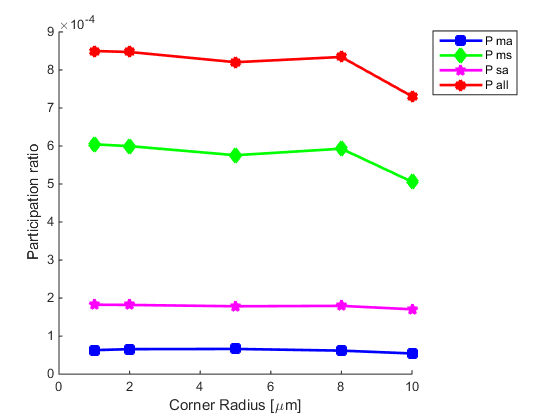
\includegraphics[scale = 0.7]{Figures/Ratio_plots/CornerRadius_legend}
 	\caption{The different participation for several corner radii. However slowly, all ratios tend to decrease with increasing radius. The ground separation distance (D) is \(20\mu m\), the finger length (L) is \(56 \mu m\), the width (W) and gap (G) of the fingers is \(20 \mu m\).}
 	\label{fig:CornerRadius}
 \end{figure}

\begin{table}
	\begin{center}
		\begin{tabular}{ | l || c | c | c | c | c |}
			\hline
			Corner radius [\(\mu\)m] & P ma & P ms & P sa & P all \\ \hline
			1 & 6.30e-05 & 6.04e-04 & 1.83e-04 & 8.50e-04 \\
			2 & 6.57e-05 & 6.00e-04 & 1.82e-04 & 8.47e-04 \\
			5 & 6.62e-05 & 5.76e-04 & 1.78e-04 & 8.20e-04\\
			8 & 6.18e-05 & 5.93e-04 & 1.80e-04 & 8.34e-04\\
			10 & 5.43e-05 & 5.06e-04 & 1.70e-04 & 7.31e-04\\
			\hline
		\end{tabular}
	\end{center}
	\caption{The participation ratios for different corner radii.}
	\label{table:ratio_cornerradius}
\end{table}

The influence of the ground plane separation distance on the participation ratios was also determined. The distance (D in figure \ref{fig:Yale_parameters2}) was changed between 10 \(\mu\)m and 200 \(\mu\)m. The fingers had a width (W) and gap (G) of \(20 \mu m\), and a length (L) of \(56 \mu m\). The resulting participation ratios can be found in table \ref{table:ratio_groundseparation} and in figure \ref{fig:SlotSize_legend} as a function of separation distance. Again, all participation ratios show a downward trend with increasing separation distance. The influence of increasing the the separation beyond 100 \(\mu\)m is very small.

 \begin{figure}
 	\centering
 	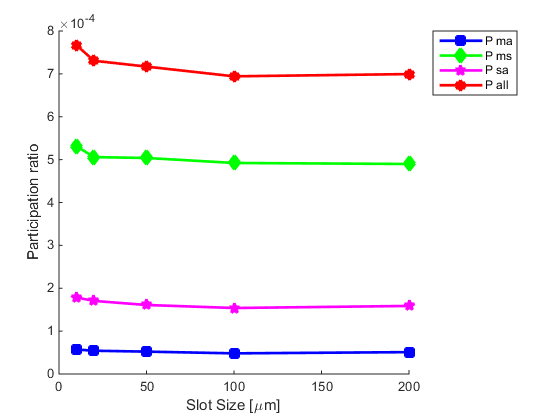
\includegraphics[scale = 0.7]{Figures/Ratio_plots/SlotSize_legend2}
 	\caption{The different participation ratios for several separation distances to the ground plane. The distance (D in figure \ref{fig:Yale_parameters2}) was changed between 10 \(\mu\)m and 200 \(\mu\)m. The fingers had a width (W) and gap (G) of \(20 \mu m\), and a length (L) of \(56 \mu m\).}
 	\label{fig:SlotSize_legend}
 \end{figure}

\begin{table}
	\begin{center}
		\begin{tabular}{ | l || c | c | c | c | c |}
			\hline
			Ground Separation [\(\mu\)m] & P ma & P ms & P sa & P all \\ \hline
			10 & 5.71e-05 & 5.31e-04 & 1.78e-04 & 7.67e-04 \\
			20 & 5.43e-05 & 5.06e-04 & 1.70e-04 & 7.31e-04 \\
			50 & 5.22e-05 & 5.04e-04 & 1.61e-04 & 7.17e-04 \\
			100 & 4.82e-05 & 4.92e-04 & 1.54e-04 & 6.94e-04 \\
			200 & 5.10e-05 & 4.90e-04 & 1.59e-04 & 7.00e-04\\
			\hline
		\end{tabular}
	\end{center}
	\caption{The participation ratios for different ground separation distances.}
	\label{table:ratio_groundseparation}
\end{table}

Looking at these results for the interdigitated qubit design it can be seen that the most significant change in participation ratios was achieved by making the fingers shorter and separating them further. Extrapolating these changes would indicate that a qubit consisting of two parallel rectangular pads would have even smaller participation ratios.

% \textit{Alternatively:}Extrapolating these changes would indicate that making the fingers ever shorter but wider would result in a qubit with even smaller participation ratios. The resulting qubit consists of two rectangular pads separated by the junction. 

\clearpage
\section{Parallel pad qubit}
The resulting qubit design can be seen in figure \ref{fig:IBM_parameters23}. It consists of two large parallel pads which are connected two smaller pads with the inductor in-between. The ground plane surrounds a square slot at a relatively large distance from the qubit. Due to its simplicity, there are fewer ways of changing the qubit. The parameters under consideration are the pad separation (S), the pad width (W), and the radius of the corners. Again, first, the influence different parameters have on the capacitance of the system was determined. Afterwards the participation ratios of different configurations were calculated.

\begin{figure}[h]
	\centering
	\begin{tabular}{c}
		\subfloat[Overview of the parallel pad qubit]{{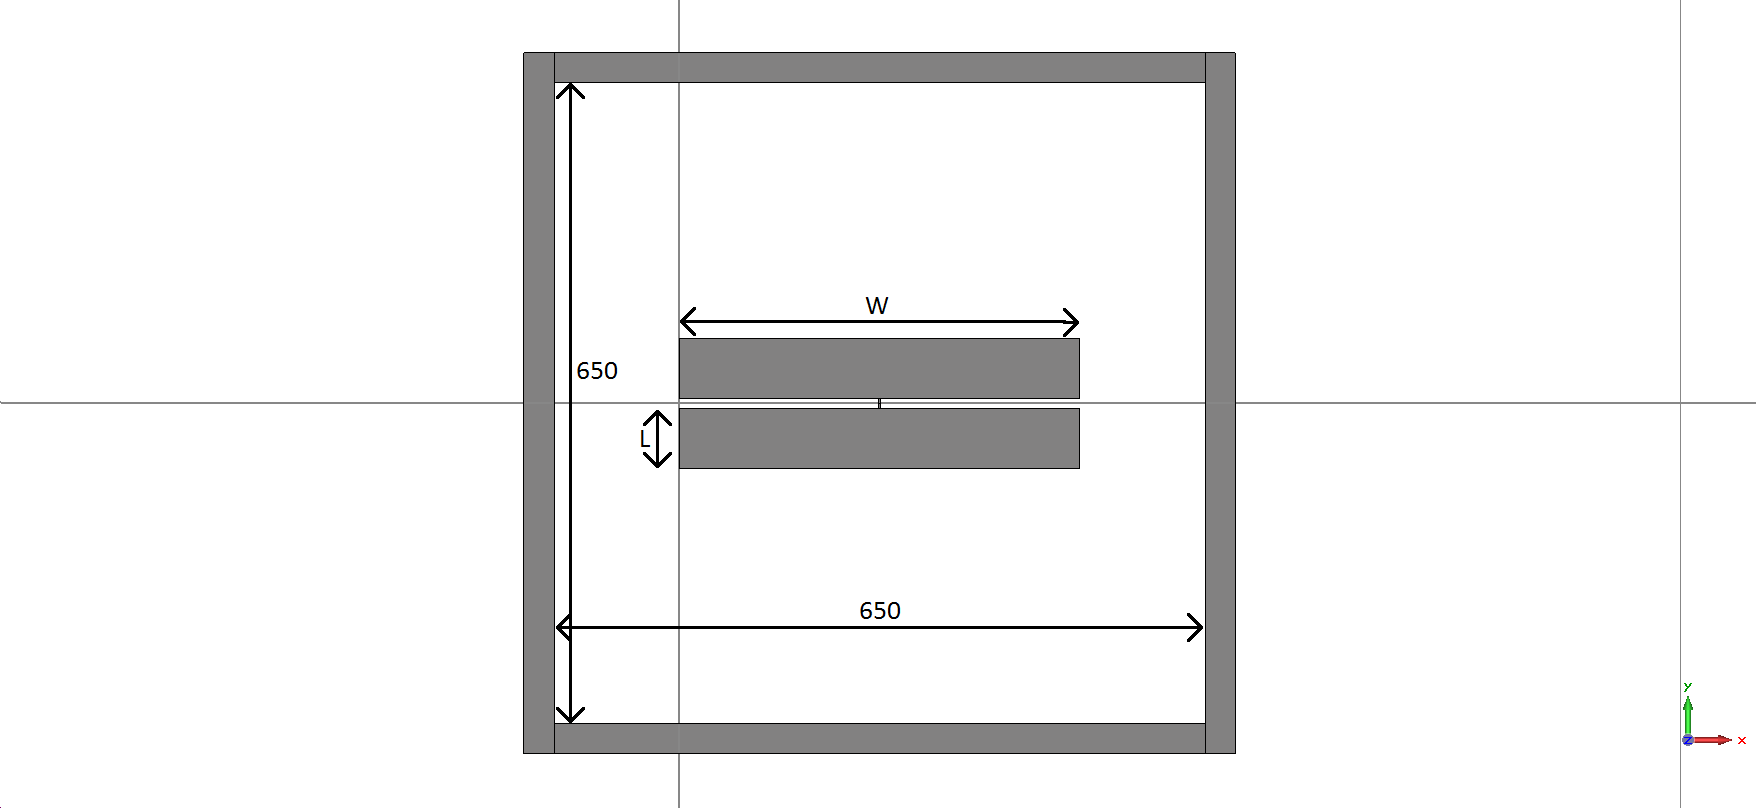
\includegraphics[width = \textwidth -15pt]{Figures/IBM_parameters3} }} \\
		
		\subfloat[Zoomed in view of the center of the qubit.]{{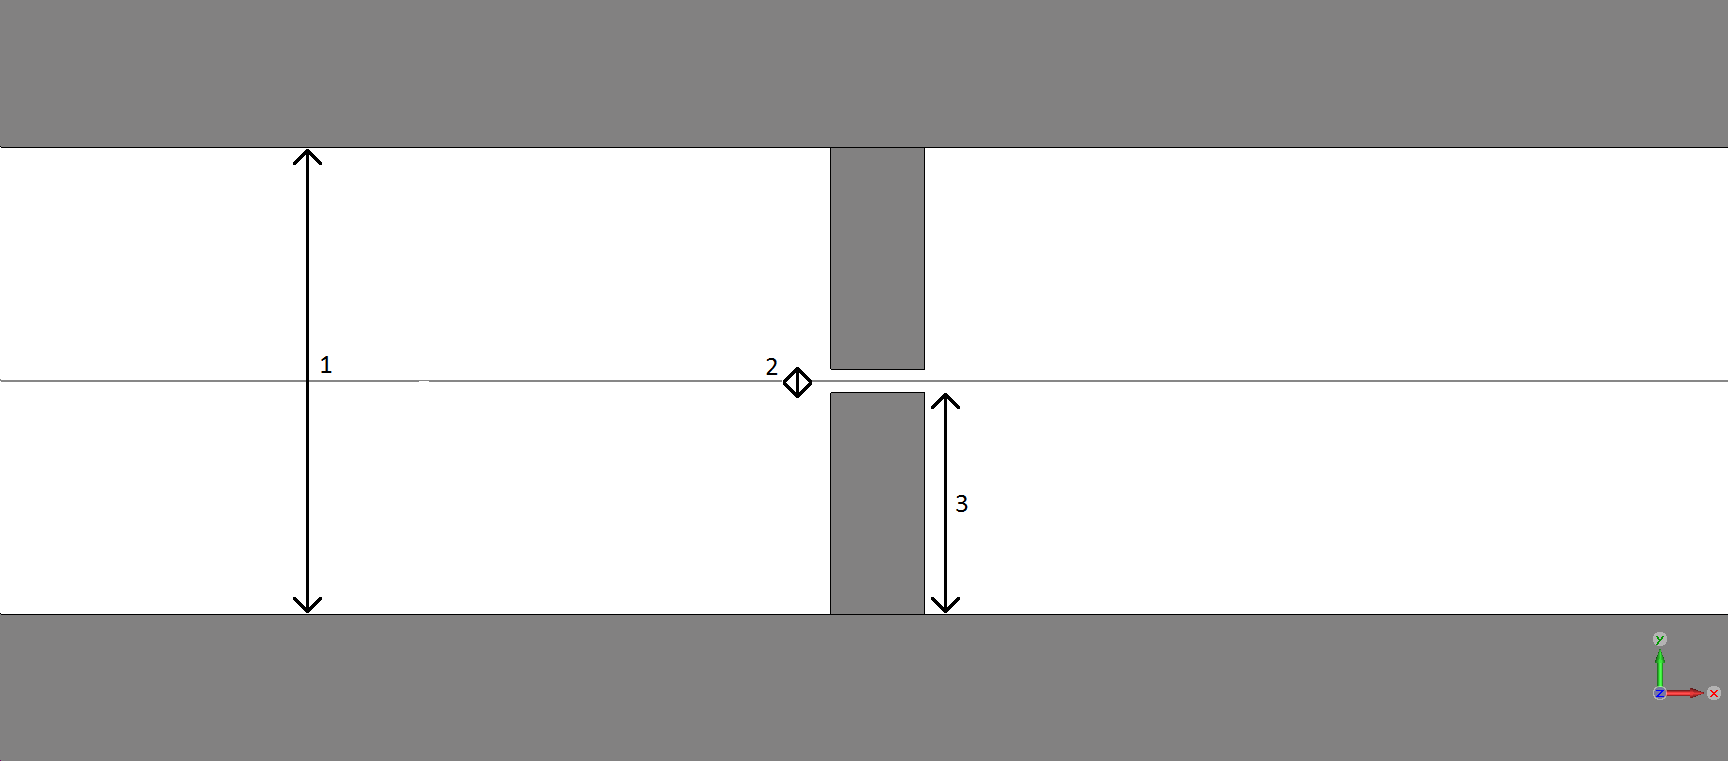
\includegraphics[width = \textwidth -15pt]{Figures/IBM_parameters2} }}
	\end{tabular}
	\caption{The parallel pad qubit design including parameters and dimensions valid for all iterations of the design. (a) W is the width of the pads, L is the length of the pad, the size of the grounded slot here is 650 \(\mu\)m. (b) 'S' is the pad separation distance. 'J' is the junction separation distance, which is 0.5 \(\mu\)m for all qubits. 'K' is the length of the junction lead which depends only on the separation distance of the qubit.}
	\label{fig:IBM_parameters23}
\end{figure}



\subsection{The capacitance}
Similar to adding extra fingers to the interdigitated qubit, widening the pad width is expected to linearly increase the capacitance of the system. The pad width was changed between 300 and 500 \(\mu\)m. The pad separation (S) is \(18 \mu m\), the pad length is \(60 \mu m\), and the slot size is \(650 \mu m\). The capacitance was plotted as a function of pad width in figure \ref{fig:IBMCapVSWidth} indeed shows a linear proportionality.

\begin{figure}
	\centering
	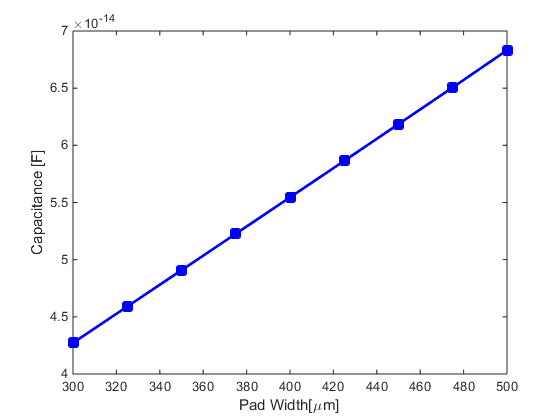
\includegraphics[scale = 0.7]{Figures/Capacitance_plots/IBMCapVSWidth}
	\caption{The capacitance of parallel pad qubits with different pad widths. The pad width (W) was changed between 300 and 500 \(\mu\)m. The pad separation (S) is \(18 \mu m\), the pad length (L) is \(60 \mu m\), and the slot size is \(650 \mu m\).}
	\label{fig:IBMCapVSWidth}
\end{figure}

The capacitance of a standard parallel plate capacitor is inversely proportional to the plate separation. Similar proportionality is expected for the parallel pad qubit system. The pad separation was set between 5 and 60 \(\mu\)m. The pad width (W) was \(450 \mu m\), the length of the pad (L) was \(60 \mu m\), and the slot size was \(650 \mu m\). The resulting capacitances as a function of pad separation distance can be seen in figure \ref{fig:IBMCapVSPadSep}.

Finally the radius of pads' corners are changed. They were set between 5 and 30 \(\mu\)m. The pad width (W) was \(450 \mu m\), the length of the pad (L) was \(60 \mu m\), the pad separation distance (S) was \(18 \mu m\), and the slot size \(650 \mu m\). The resulting capacitance as a function of corner radius is shown in figure \ref{fig:IBMCapVSCornerRadius}.

\begin{figure}[h]
	\centering
	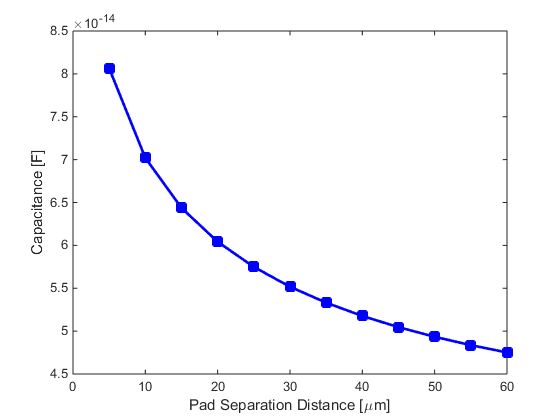
\includegraphics[scale = 0.7]{Figures/Capacitance_plots/IBMCapVSPadSep}
	\caption{The capacitance of parallel pad qubits with different pad separation distances. The pad width (W) was \(450 \mu m\), the length of the pad (L) was \(60 \mu m\), the pad separation distance (S) was \(18 \mu m\), and the slot size \(650 \mu m\).}
	\label{fig:IBMCapVSPadSep}
\end{figure}


\begin{figure}
	\centering
	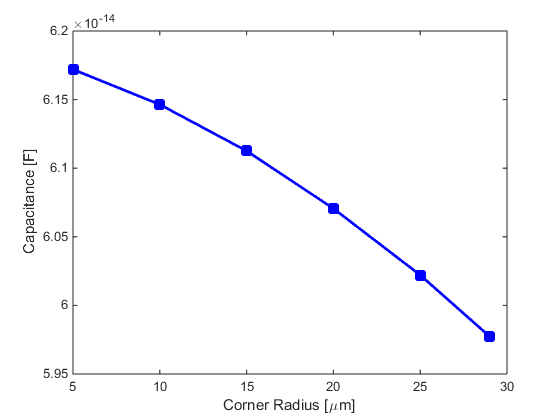
\includegraphics[scale = 0.7]{Figures/Capacitance_plots/IBMCapVSCornerRadius}
	\caption{The capacitance of parallel pad qubits with different corner radii. The pad width (W) was \(450 \mu m\), the length of the pad (L) was \(60 \mu m\), the pad separation distance (S) was \(18 \mu m\), and the slot size \(650 \mu m\).}
	\label{fig:IBMCapVSCornerRadius}
\end{figure}

\clearpage
\subsection{The participation ratios}
 %The influence of the pad separation and the pad width on the participation ratios of the layers were determined. 
 Comparing the two qubit designs; increasing the finger width (and separation) in the interdigitated qubit can be seen as increasing the pad separation and pad width in the parallel pad qubit. Therefore the participation ratios are expected to decrease when increasing pad width or separation. The influence of three parameters on the participation ratios were investigated separately: the pad separation, the pad width, and the corner radius. Contrary to what was done during the investigation of the interdigitated qubit, the resonance frequencies of all parallel pad qubits were kept equal by changing the value of the inductance (see formula \eqref{eq:ResonanceFrequency}).
 
 Starting with the pad width which was again changed between 300 and 500 \(\mu\)m. The pad separation distance (S) was \(18 \mu m\), the pad length (L) was \(60 \mu m\), and the slot size was \(650 \mu m\). Table \ref{table:ratio_IBMPadWidth} and figure \ref{fig:IBMPadWidth_legend} show the resulting ratios for different pad widths, all of them decreasing with increasing width.
 
 \begin{table}
 	\begin{center}
 		\begin{tabular}{ | l || c | c || c | c | c | c | c |}
 			\hline
 			Pad Width [\(\mu\)m] & Capacitance [\(f\)F] & Inductance [\(n\)H] & P ma & P ms & P sa & P all \\ \hline
 			300 & 42.7 & 14.0 & 4.71e-05 & 3.51e-04 & 1.08e-04 & 5.06e-04 \\
 			350 & 49.1 & 12.2 & 4.29e-05 & 3.44e-04 & 1.04e-04 & 4.91e-04 \\
 			400 & 55.5 & 10.8 & 4.27e-05 & 3.38e-04 & 1.02e-04 & 4.82e-04 \\
 			450 & 61.9 & 9.69 & 4.17e-05 & 3.32e-04 & 1.01e-04 & 4.74e-04 \\
 			500 & 68.3 & 87.8 & 4.04e-05 & 3.28e-04 & 9.92e-05 & 4.68e-04\\
 			\hline
 		\end{tabular}
 	\end{center}
 	\caption{The participation ratios of parallel pad qubits with different pad widths.}
 	\label{table:ratio_IBMPadWidth}
 \end{table}
 
 \begin{figure}
 	\centering
 	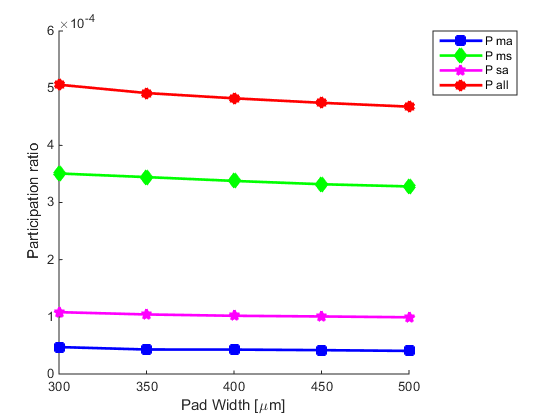
\includegraphics[scale = 0.7]{Figures/Ratio_plots/IBMPadWidth_legend}
 	\caption{The participation ratios of parallel pad qubits with different pad widths. The pad separation distance (S) was \(18 \mu m\), the pad length (L) was \(60 \mu m\), and the slot size was \(650 \mu m\).}
 	\label{fig:IBMPadWidth_legend}
 \end{figure}
 
 Secondly, the separation between the two pads was changed between 5 and 60 \(\mu\)m. The pad width (W) was \(450 \mu m\), the pad length (L) was \(60 \mu m\), and the slot size was \(650 \mu m\). The results in table \ref{table:IBMPadSep} and figure \ref{fig:IBMPadSep_legend} again show decreasing ratios for all layers with increasing separation. 
 
 \begin{table}
 	\begin{center}
 		\begin{tabular}{ | l || c | c || c | c | c | c | c |}
 			\hline
 			Pad Separation [\(\mu\)m] & Capacitance [\(f\)F] & Inductance [\(n\)H] & P ma & P ms & P sa & P all \\ \hline
 			5 & 80.6 & 7.43 & 6.42e-05 & 5.59e-04 & 1.82e-04 & 8.42e-04 \\
 			10 & 70.2 & 8.54 & 4.65e-05 & 4.26e-04 & 1.28e-04 & 6.00e-04 \\
 			20 & 60.4 & 9.92 & 4.02e-05 & 3.21e-04 & 9.67e-05 & 4.58e-04 \\
 			50 & 49.3 & 12.2 & 3.35e-05 & 2.55e-04 & 7.70e-05 & 3.65e-04 \\
 			\hline
 		\end{tabular}
 	\end{center}
 	\caption{The participation ratios of parallel pad qubits with different pad separation distances.}
 	\label{table:IBMPadSep}
 \end{table}
 
 \begin{figure}
 	\centering
 	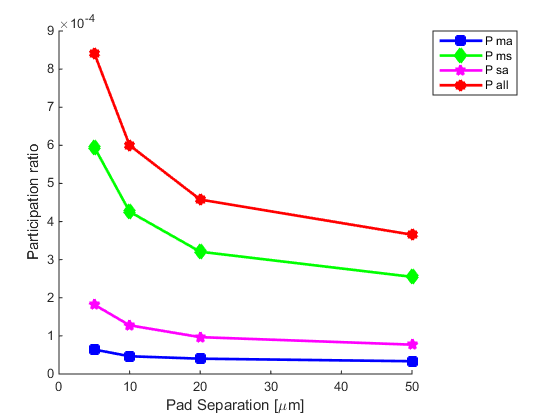
\includegraphics[scale = 0.7]{Figures/Ratio_plots/IBMPadSep_legend}
 	\caption{The participation ratios of parallel pad qubits with different pad separation distances. The pad width (W) was \(450 \mu m\), the pad length (L) was \(60 \mu m\), and the slot size was \(650 \mu m\).}
 	\label{fig:IBMPadSep_legend}
 \end{figure}
 
 Finally, the radius of the corners was changed between 5 and 30 \(\mu\)m, where a radius of 30 \(\mu\)m results in an semi-circle on the sides. The pad separation distance (S) was \(18 \mu m\), the pad length (L) was \(60 \mu m\), the pad width (W) was \(450 \mu m\) and the slot size was \(650 \mu m\). Although the resulting ratios in table \ref{table:IBMCornerRadius} and figure \ref{fig:IBMCornerRadius_legend} show a decreasing trend, the change is much less significant compared to that of the interdigitated qubit (see figure \ref{fig:CornerRadius}).
 
 \begin{table}
 	\begin{center}
 		\begin{tabular}{ | l || c | c || c | c | c | c | c |}
 			\hline
 			Corner Radius [\(\mu\)m] & Capacitance [\(f\)F] & Inductance [\(n\)H]  & P ma & P ms & P sa & P all \\ \hline
 			5 & 61.7 & 9.71 & 3.74e-05 & 3.03e-04 & 9.53e-05 & 4.35e-04 \\
 			10 & 61.5 & 9.75 & 3.56e-05 & 3.01e-04 & 9.47e-05 & 4.31e-04 \\
 			15 & 61.1 & 9.81 & 3.67e-05 & 2.98e-04 & 9.60e-05 & 4.31e-04 \\
 			20 & 60.7 & 9.88 & 3.37e-05 & 3.00e-04 & 9.51e-05 & 4.29e-04 \\
 			25 & 60.2 & 9.96 & 3.47e-05 & 2.97e-04 & 9.41e-05 & 4.26e-04 \\
 			29 & 59.8 & 10.0 & 3.49e-05 & 2.99e-04 & 9.47e-05 & 4.28e-04 \\
 			\hline
 		\end{tabular}
 	\end{center}
 	\caption{The participation ratios of parallel pad qubits with different corner radii.}
 	\label{table:IBMCornerRadius}
 \end{table}
 
 \begin{figure}
 	\centering
 	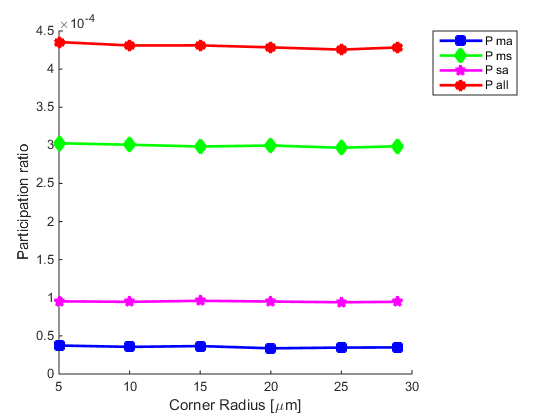
\includegraphics[scale = 0.7]{Figures/Ratio_plots/IBMCornerRadius_legend}
 	\caption{The participation ratios of parallel pad qubits with different corner radii. The pad separation distance (S) was \(18 \mu m\), the pad length (L) was \(60 \mu m\), the pad width (W) was \(450 \mu m\) and the slot size was \(650 \mu m\).}
 	\label{fig:IBMCornerRadius_legend}
 \end{figure}
 
\clearpage
\section{Further Discussion}
Finally, to explain some of the results, the simulated electric fields can be looked at. Figure \ref{fig:CornerFields} shows the absolute value of the electric field around the corners of the interdigitated (a and b) and parallel pad qubits (c and d). The electric field is less concentrated when the corners are rounded. It appears these highly concentrated electric fields at the corners are a cause for higher participation ratios. The reduction of the participation ratios is most apparent for the interdigitated qubit which simply has more corners.

 \begin{figure}
 	\begin{tabular}{c c}
 		\subfloat[Interdigitaded, finger slightly rounded]{{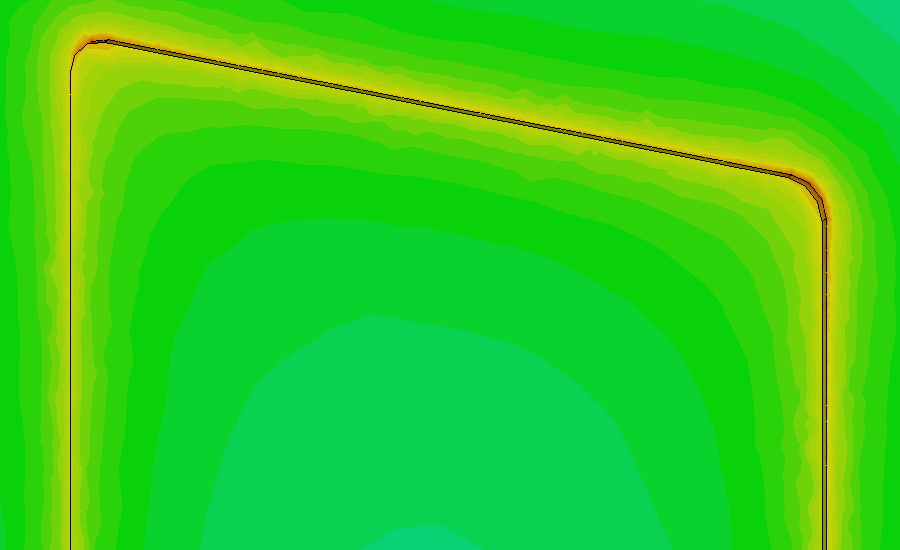
\includegraphics[width = -15pt + \textwidth/2]{Figures/Fields/slightly_rounded_zoomed_cropped} }} & \subfloat[Interdigitaded, finger fully rounded]{{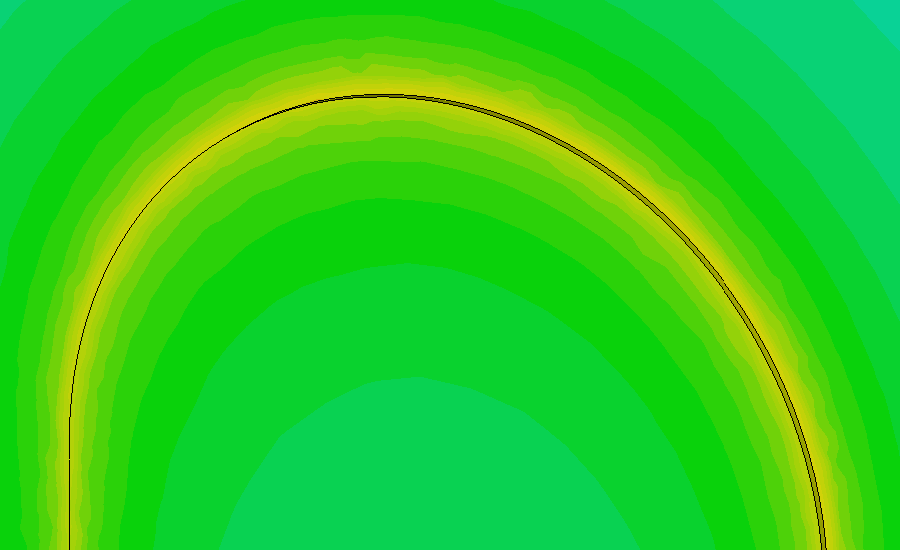
\includegraphics[width = -15pt + \textwidth/2]{Figures/Fields/fully_rounded_zoomed_cropped} }} \\
 		\subfloat[Parallel pad, sharp corner]{{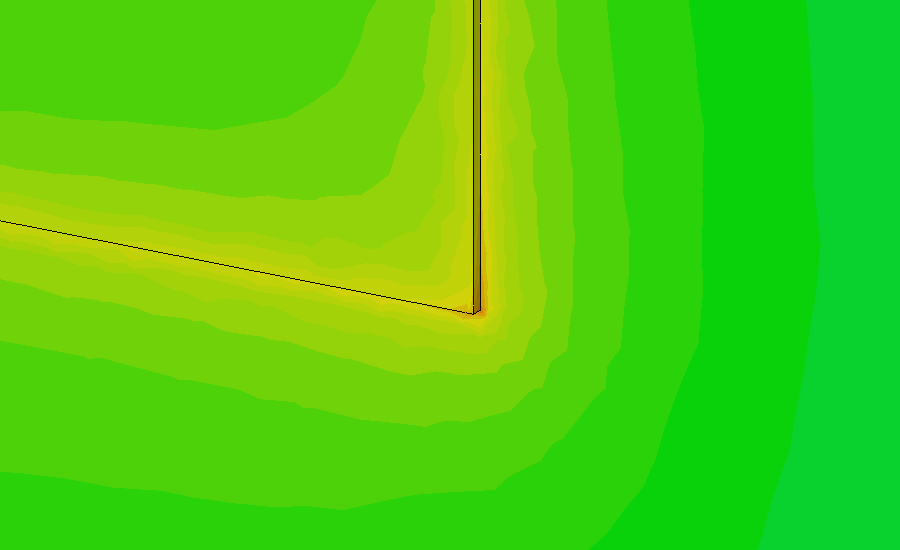
\includegraphics[width = -15pt + \textwidth/2]{Figures/Fields/IBM_sharp_corner_cropped} }} & \subfloat[Parallel pad, rounded corner]{{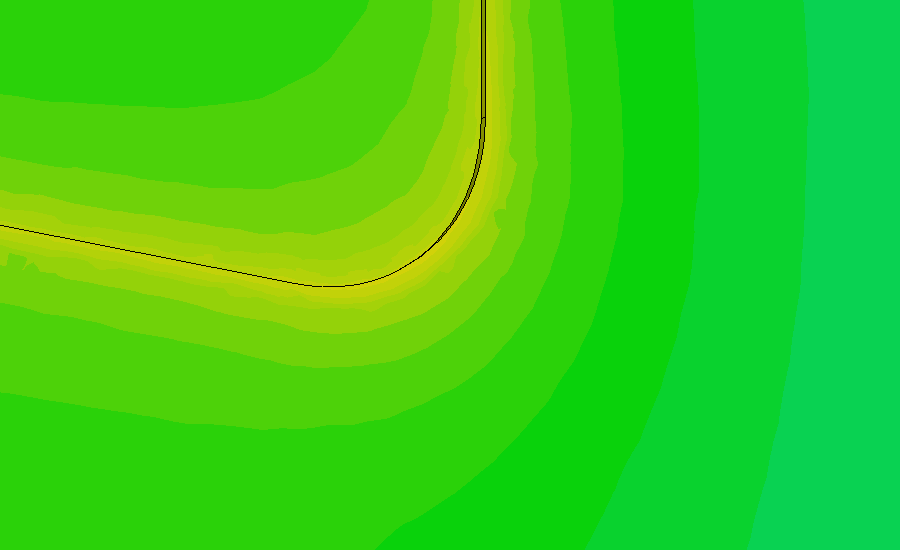
\includegraphics[width = -15pt + \textwidth/2]{Figures/Fields/IBM_rounded_corner_r5_cropped} }}
	 \end{tabular}	
 	\centering	
 	\caption{The absolute value of the electric field in the area around corners. The rounding of the corners results in less concentrated electric fields.}
 	\label{fig:CornerFields}
 \end{figure}

 
Figure \ref{fig:PadSeparationFields} shows the electric field on a cross-section of the parallel pad qubit with different pad separation distances, 50 \(\mu\)m away from the junction. For both depicted qubits the intensity of the electric field is greatest on the edges between the two pads. When the pads are close to each other, as in (a) and (c), the field near the edges is more intense. As a result the participation ratios of all lossy layers is lower when the pads are further apart.

\begin{figure}
 	\begin{tabular}{c c}
 		\subfloat[Separation distance 5 \(\mu\)m]{{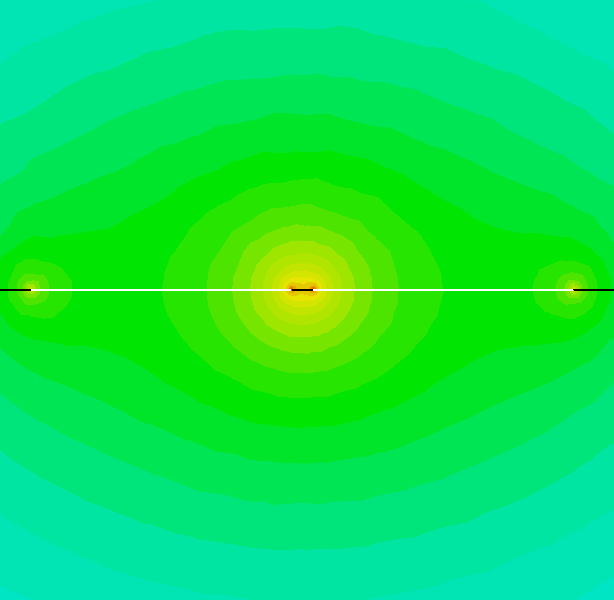
\includegraphics[width = -15pt + \textwidth/2]{Figures/Pad_sep_Fields/sep_5_semizoomed_cropped} }} & \subfloat[Separation distance 50 \(\mu\)m]{{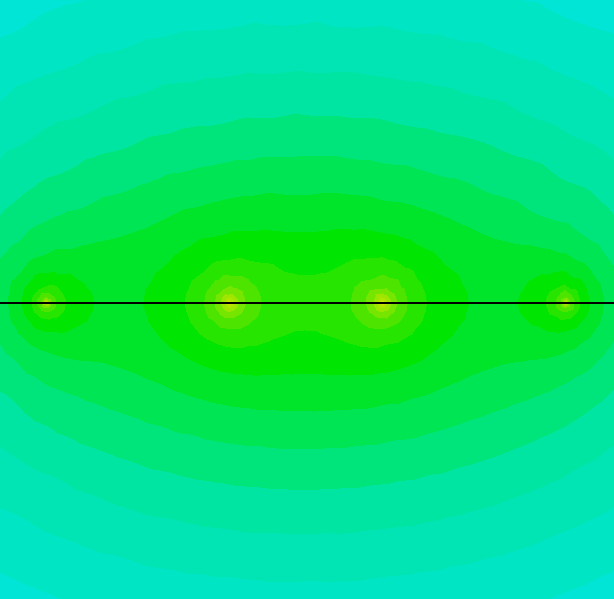
\includegraphics[width = -15pt + \textwidth/2]{Figures/Pad_sep_Fields/sep_50_semizoomed_cropped} }} \\
 		\subfloat[Separation distance 5 \(\mu\)m, zoomed]{{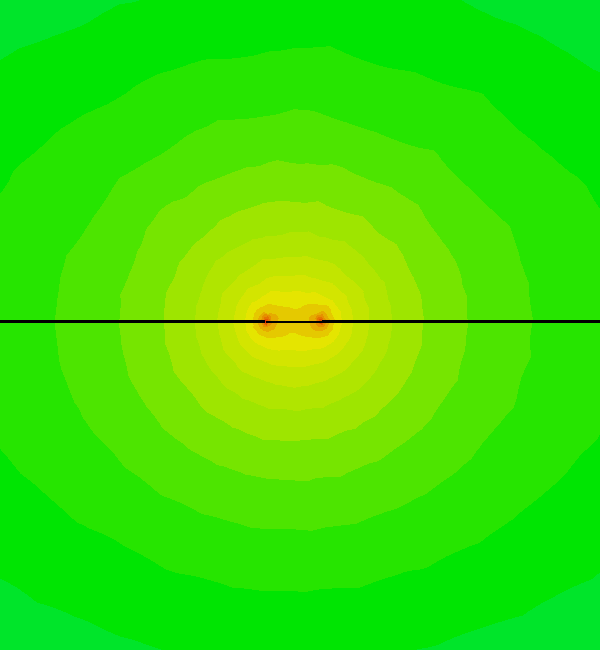
\includegraphics[width = -15pt + \textwidth/2]{Figures/Pad_sep_Fields/sep_5_zoomed_cropped} }} & \subfloat[Separation distance 50 \(\mu\)m, zoomed]{{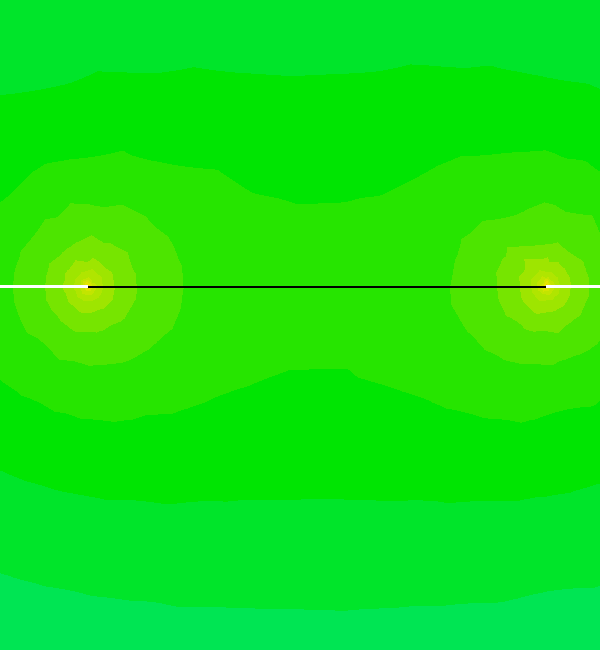
\includegraphics[width = -15pt + \textwidth/2]{Figures/Pad_sep_Fields/sep_50_zoomed_cropped} }}
 	\end{tabular}	
 	\centering	
 	\caption{The absolute value of the electric field in the area surrounding the pads. The location of the pads is depicted in white. The intensity of the field in the area between the pads is significantly lower when the separation distance is increased.  }
 	\label{fig:PadSeparationFields}
 \end{figure}
 
%\section{Conclusion} %Grafieken niet in de conclusie! hier geen nieuwe informatie geven!
%To explain these results the actual electric field can be looked at. Figure \ref{fig:} shows a comparison of the electric field intensity belonging to parallel pad qubits with a width of 300 and 500 \(\mu\)m. \todo{Explain differences in field intensity}.
% 
%Next, figure \ref{fig:} shows a comparison of the electric field intensity belonging to parallel pad qubits with a separation distance of 5 and 60 \(\mu\)m, a cross-section is also included. \todo{Explain differences in field intensity}.
% 
%Finally, figure \ref{fig:} shows a comparison of the electric field intensity belonging to both interdigitated and parallel pad qubit having partial of fully rounded corners. The difference is especially noticeable for the interdigitated qubits. \todo{Explain differences in field intensity}.
  




    